\section{Introduction} \label{sec:intro}


\section{Design goals} \label{sec:design}


\section{The Faro Framework} \label{sec:faro}

\faro has adopted a modular and extensible design that can be configured  to run any subset of metrics on any subset of data products, e.g., a  subset of the realtime metrics computed on a single exposure. 
Two main components form the basis of the \faro framework;  a collection of \texttt{Task}s that compute specific metric values, and a set of base classes that handle data i/o for various types of input data units corresponding to the granularity of metric computation, e.g., per-detector, per-visit, per-patch, per-tract. 
\faro builds upon much of the existing infrastructure of the LSST Science Pipelines, in particular the ``Generation 3'' middleware, including the Data Butler and Task Framework\footnote{\url{https://pipelines.lsst.io/modules/lsst.pipe.base/task-framework-overview.html}}\cite{dmtn-229}, and the LSST verification framework\cite{SQR-019}. 
The LSST Data Butler (hereafter the ``Butler'') provides an abstracted data access interface that is used to read and write data without having to know the details of file formats or locations.
The Butler organizes data, both raw and processed, into data repositories.
A \texttt{Task} is a reusable unit of code in the LSST science pipelines infrastructure that is used to process data.
Each Task has a specialized configuration object attached to it and provides a \texttt{run()} method that implements the algorithm to execute. 
Each \faro metric has an associated \texttt{Task} class that implements the mathematical algorithm to compute the scalar metric value on the input data.
The LSST Verification Framework, \texttt{lsst.verify}, is a framework for making verification measurements in the LSST Science Pipelines.
\faro takes as input catalog data products generated by the LSST Science Pipelines\footnote{The LSST science pipelines produce catalog data products both in FITS and parquet file format. \faro works exclusively with with parquet formatted data.} stored in a Butler repository, 
%  but in principle could use any data product available in a Butler repository, including images, 
 and computes scalar performance metrics on them. 
The resulting metric values
% \footnote{The result of computing a given metric on some set dataset.} 
are persisted in the same Butler repository alongside the input data products, each with an associated searchable data identifier\footnote{A dict-like identifier for data usable across multiple Butler collections and DatasetTypes.} as \texttt{lsst.verify.Measurement} objects.

\subsection{Analysis Contexts} \label{ssec:contexts}

An analysis context defines the type of input data unit corresponding to the granularity of metric computation, e.g per-detector, per-visit, per-patch or per-tract.
\faro supports metric calculation for a multiple analysis contexts, that is, the same mathematical function can be called in a different analysis context to produce a different metric value. 
For example, the residual PSF ellipticity correlation metrics can be computed on a per-visit or per-tract analysis context. 
For some metrics, only certain analysis contexts make sense and often the choice of analysis context will be dictated by statistics, e.g a small 1\degsq CI dataset may not contain enough data to compute some metrics on a per-tract level. 
\faro allows users to easily define a new analysis contexts for their particular science need. 

The following analysis, corresponding to analysis contexts  are currently supported in \faro:
\begin{itemize}
\item per-detector source catalogs i.e., single-visit detections
\item per-visit source catalogs i.e., single-visit detections
\item per-patch object catalogs i.e., coadd detections both per-band and multi-band
\item per-tract object catalogs i.e., coadd detections, both per-band and multi-band input
\item per-patch matched source catalogs, i.e., set of single-visit detections of the same objects, both single band and multi-band input
\item per-tract matched source catalogs, i.e., set of single-visit detections of the same objects 
\end{itemize}


\subsection{Base Classes} \label{ssec:baseclasses}

\faro provides a set of base classes corresponding to the various analysis contexts described above that use the \texttt{PipelineTask} framework to build a quantum graph\footnote{A data structure that represents a concrete workflow generated from a Pipeline.} and interact with Butler for data i/o.
By abstracting the data i/o, developers can focus on the algorithmic implementation of the metrics. 
The primary base classes in the lsst.faro package are \texttt{CatalogMeasurementBaseConnections}, \texttt{CatalogMeasurementBaseConfig}, and \texttt{CatalogMeasurementBaseTask}, each of which inherits from  \texttt{MetricConnections}, \texttt{MetricConfig}, and \texttt{MetricTask}, in the \texttt{lsst.verify} package respectively, and adds additional general functionality for computing science performance metrics based on Source and Object catalog inputs. 
Once the analysis context base class is defined, developers can implement metrics by creating a dedicated \texttt{Task} that will operate on in-memory python objects. 
Unlike many other \texttt{Task}s  in the LSST science pipelines, such as fitting a WCS or detecting sources on an image, \texttt{Task}s for metric computation with \faro work with in-memory python objects.
The base classes for the various analysis contexts are located in the \texttt{python/lsst/faro/measurement} directory.

\subsection{Stages of Metric Computation} \label{ssec:stages}

Metric computation with \faro proceeds through three stages:
\begin{enumerate}
\item \textbf{Preparation:}  any intermediate data products that are needed as input to the subsequent measurement step are assembled and persisted in the Butler.	
\item \textbf{Measurement:} the metric \texttt{Task} is run to compute a measurement for each unit of data (i.e., a quantum of processing with a particular a dataId for the output measurement). Measurements are stored as \texttt{lsst.verify.Measurement} objects.
\item \textbf{Summary:}  a single scalar summary statistic, e.g a mean, median, etc is generated from the collection of input measurements computed in the measurement stage.  Summary statistics are stored as \texttt{lsst.verify.Measurement} objects and persisted in the Butler.
\end{enumerate}
Not all metrics will necessarily have a  preparation stage as there may be no additional intermediate data products needed to compute the metric than those generated as part of the pipelines processing, however all must have a measurement and summary stage. 

Take as an example the photometric repeatability metric, PA1, which measures the RMS photometric repeatability of bright non-saturated unresolved point sources in a single filter.
During the preparation stage, a matched source catalog is created for each tract and band that matches source detections in individual visits that correspond to the same physical astronomical object\footnote{LSST defines an Object as an astrophysical physical object, e.g a star, galaxy or asteroid, and a Source as a  single detection of an astrophysical object in an image. The association of Sources that are non-moving lead to Objects; the association of moving Sources leads to Solar System Objects.}. 
During the measurement stage, for each tract and band, the matched catalog computed and stored in the preparation stage is loaded into memory and used to compute the RMS scatter of fluxes for a single astrophysical object. 
In the final summary stage, the measurements for the ensemble of individual tracts computed in the measurement stage are loaded to compute a median summary statistic per band. 
This final summary statistic characterizes the overall performance for the dataset per band and is stored as an \texttt{lsst.verify} object in the Butler. 


\subsection{Processing Pipelines} \label{ssec:pipelines}


\section{Adding a  Metric} \label{sec:add}


\section{Tracking and Visualization} \label{sec:tracking}


\section{Faro Applications} \label{sec:applications}

\subsection{Monitoring Science Pipelines Performance} \label{ssec:monitoring}

\subsubsection{Precursor datasets} \label{sssec:datasets}

\subsubsection{Continuous Integration}\label{sssec:ci}

\subsubsection{Software Release Characterization } \label{sssec:characterization}


\begin{figure}[htb]
  \centering
  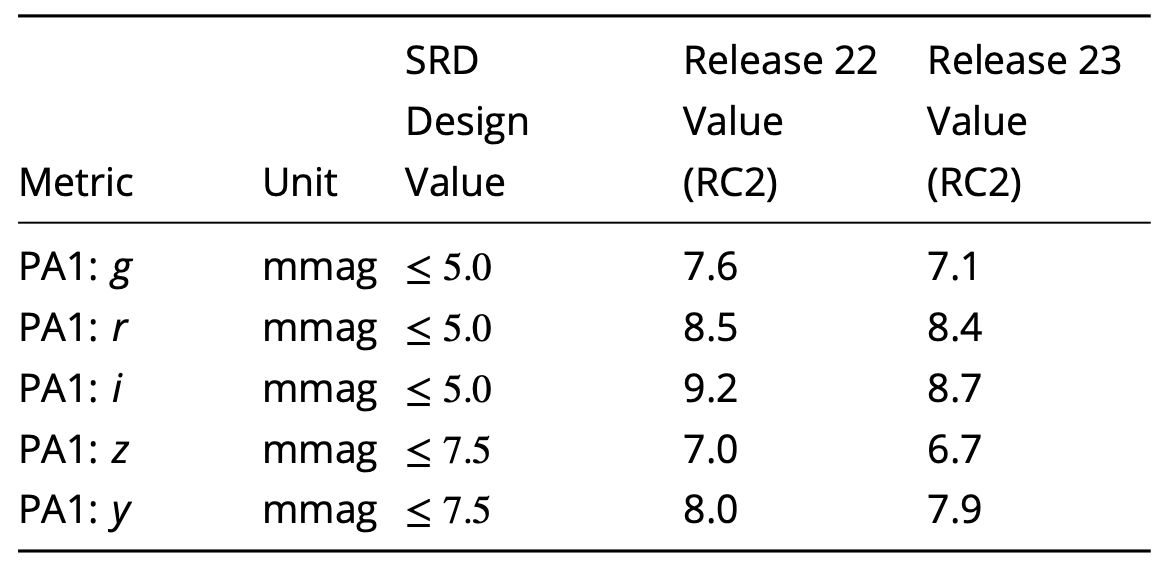
\includegraphics[width=0.45\textwidth]{figures/cmr_r23_photometric_metrics} 
  \hspace{0.5cm}
  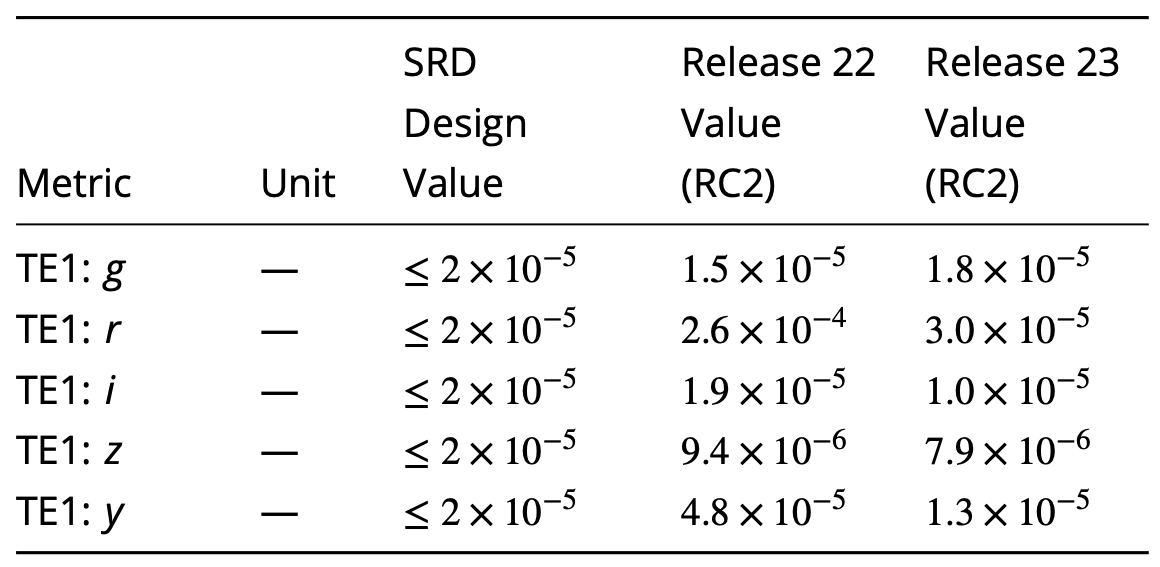
\includegraphics[width=0.45\textwidth]{figures/cmr_r23_ellipticity_metrics}
  \par\medskip % force a bit of vertical whitespace
  \caption{Excerpt from the  LSST Science Pipelines major Release 23 Characterization Metric Report on the HSC RC2 dataset. Metric values are compared with those of the previous release of the science pipelines and with the  design values from the LSST Science Requirements document SRD.}
  \label{fig:cmr_r23}
\end{figure}

\subsection{Rubin Auxiliary Telescope} \label{ssec:auxtel}

\subsection{Rubin Data Previews} \label{ssec:datapreviews}

\section{Current Status and Future Development} \label{sec:future}

\section{Conclusions} \label{sec:conclusions}